\renewcommand{\chaptername}{Chapitre}
\label{part:Analyse du Problème}
\chapter{Host Organization \& Project Context}

% Chapter 1
A concise overview of Theodo’s history, mission, core values, and culture, along with the thorough hiring and onboarding processes that shaped my internship experience

\section{Introduction}

This opening chapter establishes the comprehensive foundation for understanding both the organizational environment and project context that shaped my end-of-study internship experience. The chapter bridges the gap between the professional setting at Theodo Morocco and the specific challenges of modernizing the National Sports Federation's critical infrastructure, demonstrating how organizational culture and project requirements aligned to create an ideal learning environment.

The first section introduces Theodo Morocco, the dynamic software consultancy where I conducted my internship. From its origins as Nimbleways in 2017 to its integration into the international Theodo Group in 2019, the company has established itself as a key player in delivering high-quality digital solutions across North Africa. Theodo's core values—rigor, pragmatism, eagerness to progress, and team spirit—directly influenced how the FDME project was approached, executed, and delivered. Understanding these values is essential for appreciating the methodical yet agile approach that characterized every aspect of the project.

The second section presents the specific project context that brought together Theodo's expertise with the federation's urgent modernization needs. The National Sports Federation, representing one of Europe's most significant sporting institutions, manages over 500,000 licensed members across 2,300 clubs and orchestrates more than 70,000 matches annually. This massive operational scale demanded sophisticated digital infrastructure to maintain standards of fairness, transparency, and operational excellence throughout the national handball ecosystem.

The third section analyzes the legacy Electronic Match Sheet (FDME) system that had served as the backbone of match reporting for nearly fifteen years. Originally developed in the early 2010s with Windows desktop applications and limited web interfaces, the system had accumulated critical technical limitations including platform compatibility issues, connectivity resilience problems, user interface constraints, and performance degradation under load. These technical bottlenecks translated into tangible operational challenges affecting referees, coaches, administrators, and volunteers nationwide.

Together, these sections establish how Theodo's methodical approach to software delivery perfectly matched the federation's need for reliable, user-centered solutions capable of supporting distributed operations across thousands of venues with varying technical capabilities. The chapter demonstrates how organizational excellence and project complexity intersected to create an environment ideal for applying cutting-edge software engineering practices to challenges of national significance.

% Placeholder for Figure: Theodo logo
\begin{figure}[h]
\centering
\vspace{1em}
\includegraphics[width=8cm]{./images/theodo_Logo.png}
\caption{Theodo Logo}
\end{figure}

\section{Host Organization}

In 2019, Nimbleways became part of the Theodo Group, an international startup studio officially known as M33. Theodo brings together several specialized entities, each with strong technical capabilities in key domains such as finance, health, artificial intelligence, public services, cloud infrastructure, and software craftsmanship. This collaborative ecosystem includes divisions like Theodo FinTech, Theodo Data \& AI, Theodo Cloud, Theodo Apps, Theodo HealthTech, and Theodo GovTech—each addressing unique verticals while upholding a shared culture of delivery excellence.

Theodo is built on a Lean-inspired culture, emphasizing continuous improvement, team empowerment, and rapid delivery of business value. Its mission is to co-build innovative digital products hand-in-hand with clients, while ensuring a high standard of software quality and sustainability. Teams operate in close alignment with stakeholders, applying agile methodologies and a pragmatic, impact-oriented mindset to drive measurable outcomes.

Thanks to this integration, the former Nimbleways—now Theodo Morocco—benefits from the group’s global reach and knowledge-sharing culture while continuing to grow its influence in North Africa. The Casablanca-based team has successfully delivered over 70 digital products across sectors such as banking, payments, insurance, health, and sports. With a strong recommendation rate and several international collaborations, Theodo Morocco now serves as a key delivery hub for the group.


% Placeholder for Figure: Theodo Groupe ilustration
\begin{figure}[h]
\centering
\vspace{1em}
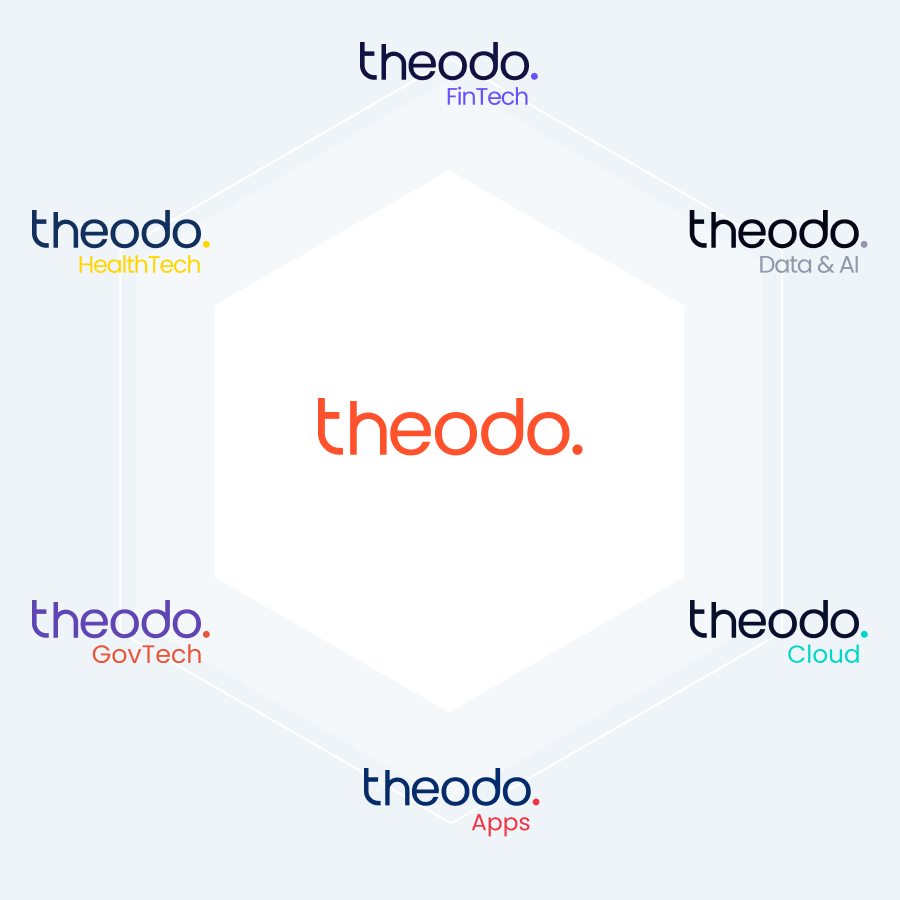
\includegraphics[width=8cm]{./images/theodo-group.png}
\caption{Theodo Groupe illustration}
\end{figure}


\section{Values \& Mission}

The core values at \textit{Theodo} play a crucial role in shaping the work culture and
guiding the approach to delivering high-quality solutions. These values ensure the maintenance of professionalism, foster continuous improvement, and prioritize teamwork in all projects.

\subsectionillustration

Rigor at \textit{Theodo} signifies diligence and carefulness in client work. Clients expect the highest standards of professionalism and diligence, which are upheld by being reliable and taking clear steps to ensure successful outcomes. Mediocrity is not accepted. To maintain this standard, the team employs practices such as writing daily to-do lists, conducting regular client recaps, holding review meetings, and systematically documenting learnings. Formalism in processes ensures consistent and high-quality results.


\subsection{Pragmatism}

Pragmatism is about getting things done efficiently while eliminating waste.
\textit{Theodo} solves problems using structured methods rather than seeking individual heroism. Discussions are based on concrete items, avoiding abstract philosophical debates. This practical approach ensures problem-solving processes are effective and focused on achieving tangible outcomes. By focusing on practical solutions, efficiency and productivity in projects are maximized.


\subsection{Eagerness to Progress}

\textit{Theodo} is committed to continuous improvement and stepping out of comfort zones. The environment encourages asking for help and viewing problems as opportunities to learn and enhance expertise. The team actively seeks learning opportunities and does not make excuses. This eagerness to progress is exemplified by practices such as the Andon system, which highlights and addresses issues in real-time, allowing for immediate learning and improvement.


\subsection{Team Spirit}

Team spirit at \textit{Theodo} means prioritizing the team's interest over personal
interests. Team members challenge each other to maintain high standards and do not tolerate average work. The focus is always on the team's objectives, with personal tasks taking a backseat to team goals. This collective approach ensures a consistent strive for excellence and mutual support. By fostering a strong team spirit, a collaborative and high-performing work environment is created. These values are integral to \textit{Theodo}' identity and operations. They guide actions, shape interactions with clients and colleagues, and ensure the consistent delivery of exceptional results.

\textit{Theodo} is dedicated to the mission of achieving quality software, made in Morocco. This mission underscores their commitment to developing high-caliber digital solutions that cater to the varied needs of their clients, ranging from startups to large corporations and government entities. By leveraging the expertise of local talent and adhering to stringent standards of professionalism and diligence, \textit{Theodo} ensures that each project they undertake is executed with precision and excellence. The company's focus on producing top-tier software aims to position Morocco as a leading hub for innovative software development, showcasing the region's capability to deliver world-class technology solutions. Through this mission, \textit{Theodo} not only
contributes to the digital transformation of their clients but also promotes the growth and recognition of the Moroccan tech industry on a global scale.

% Placeholder for Figure: Awards received by Nimbleways from ChooseMyCompany 
\begin{figure}[h]
\centering
\vspace{2em}
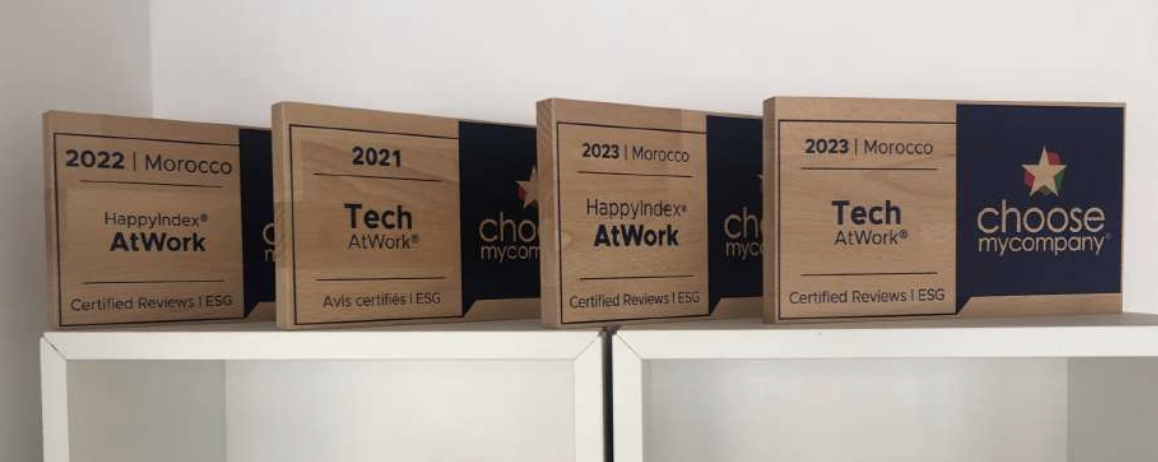
\includegraphics[width=0.7\linewidth]{images/theodo-awards.png}
\caption{Awards received by Theodo from ChooseMyCompany for excellence in workplace satisfaction and technology environment in 2021, 2022, and 2023.}
\end{figure}



\section{Hiring Process}

Securing an internship opportunity at \textit{Theodo} was an exhilarating journey that encompassed various stages of assessment and interaction. Each step of the process was meticulously designed to evaluate not just my technical prowess but also my personal attributes and aspirations. Let me walk you through the immersive experience of the \textit{Theodo} interview process.
It all began with the initial step, a multiple-choice questionnaire (MCQ). This phase tested my proficiency in full-stack development, object-oriented programming (OOP), data structures, as well as my familiarity with programming languages such as C and Java. The MCQ, held on Wednesday, 18th October 2024, provided a comprehensive overview of my technical knowledge and aptitude.

Following the MCQ, I progressed to the second stage: the HR exchange. Scheduled for Tuesday, 5th November 2024, this segment provided a platform for me to not only showcase my technical competencies but also to delve into personal anecdotes and experiences. Through a series of questions, I had the opportunity to introduce myself, share insights into my motivations for pursuing a career in software engineering, and narrate projects I had undertaken beyond academic endeavors. Moreover, I discussed instances where I encountered challenges and elucidated on the strategies employed to overcome them, thereby highlighting my problem-solving abilities. Additionally, the HR exchange allowed me to inquire about Theodo and gain deeper insights into the company culture and ethos.

The subsequent phase, a logic test conducted via Google Meet on Monday, 11th
November 2024, presented a captivating puzzle that tested my analytical and critical thinking skills. The scenario posed a thought-provoking challenge rooted in logic and reasoning, culminating in a stimulating exercise that showcased my ability to tackle complex problems methodically.

As I progressed further, I encountered the Test-Driven Development (TDD) interview, scheduled for Wednesday, 20th November 2024. This segment entailed the application of the Red-Green-Refactor approach to the Bowling Game Kata, emphasizing the importance of iterative development and test-driven methodologies. Through this exercise, I demonstrated not only my technical proficiency but also my adherence to best practices in software development.

The subsequent stage involved an interview with the Chief Technology Officer (CTO) via Google Meet on Wednesday, 2nd December 2024. This segment encompassed a wide array of topics ranging from fundamental data structures like LinkedLists and binary trees to advanced concepts such as immutability and design patterns. Through coding challenges and theoretical inquiries, I elucidated my understanding of core concepts while showcasing my problem-solving abilities and technical acumen.

The penultimate phase of the interview process involved a face-to-face interaction with the COO at \textit{Theodo} headquarters on Friday, 6th December 2024. This segment provided an opportunity for me to present myself holistically, discussing not just my academic and professional pursuits but also my extracurricular activities and personal aspirations. Additionally, the COO interview facilitated a candid dialogue wherein I gained insights into \textit{Theodo}' vision and ethos while articulating my own career aspirations and alignment with the company's values.

Finally, the journey culminated in a comprehensive tour of the workspace and a fruitful discussion with \textit{Theodo}' head of growth, wherein I had the opportunity to address any lingering queries and solidify my understanding of the company's culture and growth trajectory.

In retrospect, the \textit{Theodo} internship interview process was not just an evaluative exercise but a transformative journey that provided valuable insights, fostered personal growth, and affirmed my passion for software engineering. Through each phase, I embraced challenges, showcased my skills, and forged meaningful connections, culminating in a rewarding experience that laid the foundation for future endeavors. As I embark on this new chapter with \textit{Theodo}, I am filled with excitement and gratitude for the opportunity to contribute, learn, and grow within this dynamic and innovative organization.


\section{Onboarding Processes}

Starting my internship at \textit{Theodo} was an immersive and exhilarating experience, designed to integrate new team members seamlessly into the company’s dynamic environment. The onboarding process was comprehensive, fostering both professional growth and personal connections while ensuring that interns were well-equipped to contribute effectively from day one.

The journey began with the Asakai meeting, a hallmark of \textit{Theodo}' collaborative culture. On the very first day, I joined fellow interns in introducing ourselves to the team. The meeting was a vibrant mix of energy and enthusiasm, as each team showcased their progress. This initial introduction not only made us feel welcome but also provided insight into the ongoing projects and the company’s dynamic workflow. The morning concluded with a delightful breakfast in the office kitchen, offering a perfect opportunity to engage informally with team members and further build rapport.

\textit{Theodo} extended a warm welcome with some thoughtful swag, including branded merchandise that made us feel part of the team. We were also provided with official organization emails, granting access to professional accounts and the company's Notion page. This digital workspace was crucial for our onboarding, presenting tasks organized on a Kanban board, which we dived into for the rest of the day. These initial tasks were designed to familiarize us with the company’s tools and methodologies, setting a solid foundation for our roles.

The onboarding project provided a hands-on experience that was both challenging and rewarding. I delved into frontend development using Next.JS, exploring styled components alongside the MUI component library. Implementing the Redux pattern to dynamically toggle the theme mode and mastering various React hooks such as useState, useEffect, useRef, and useMemo were significant milestones. Additionally, creating custom hooks and leveraging existing ones from \textit{Theodo}’ boilerplate enhanced my understanding of efficient coding practices. An exciting aspect of this phase was testing UI components using the React Testing Library and Jest, culminating in the successful implementation of the landing and sign-in pages complete with all
necessary UI components.

Transitioning to backend development, my primary focus was on understanding and
utilizing the Spring Boot boilerplate. Initially, this posed a challenge, but as I became more familiar with its architecture, my productivity increased. The task of refactoring the existing codebase to align with the onboarding project’s requirements was meticulous but crucial, involving not just revamping code segments but also fine-tuning tests to ensure seamless functionality.

Throughout the onboarding process, I participated in several sessions and workshops that were pivotal for my professional development. Sessions with \textit{Kabous Nada} covered critical topics such as Andon, Perfect User Story, and Daily Mail, enhancing my understanding of effective project management and communication. Dojos and workshops provided deeper insights into various technical and methodological aspects, from standards of delivery to technical refinement and ticket manufacturing flow.

The onboarding process at \textit{Theodo} was a comprehensive and enriching experience. It was meticulously designed to integrate new interns into the company culture, equip them with essential tools and knowledge, and provide opportunities for meaningful contributions. This process not only prepared me for my role as a Software Engineer but also fostered a sense of belonging and collaboration, essential for my professional growth and success within the company.

Having established the organizational foundation and my integration into Theodo's collaborative environment, the following sections examine the specific project context and challenges that defined the FDME modernization initiative.

\newpage

\section{Project Context}

\subsection{Federation Structure and Scale}

The federation operates through a sophisticated hierarchical structure that reflects the diverse nature of national handball. At the national level, the federation oversees elite competitions including the Premier Men's Professional League, Elite Women's Professional League, and various national cup competitions. These high-profile events generate significant media attention and commercial value, requiring precise data management for broadcasting partners, sponsors, and regulatory compliance.

Regional committees manage intermediate-level competitions and coordinate with departmental committees who oversee local leagues and youth development programs. This three-tier structure ensures that handball remains accessible at the grassroots level while maintaining pathways for talented players to progress to elite levels. Each level has distinct reporting requirements, match formats, and regulatory frameworks that the FDME system must accommodate.

The federation also manages specialized competitions including beach handball, wheelchair handball, and corporate handball leagues, each with unique rules, scoring systems, and participant categories. This diversity demands a flexible, extensible platform capable of adapting to different sporting contexts while maintaining data consistency and integrity across all formats.

\subsection{Stakeholder Diversity and Workflow Complexity}

The FDME system serves an remarkably diverse user base, each with distinct needs, technical capabilities, and operational contexts:
Match Officials and Referees: Approximately 8,000 certified referees nationwide use the FDME during live matches. They require intuitive interfaces for real-time event recording, clear visual feedback for rule enforcement, and reliable offline operation since many gymnasiums lack stable internet connectivity. Referees often work under intense pressure during high-stakes matches, making usability and reliability paramount concerns.

\textbf{Club Administrators and Secretaries}: Volunteer administrators at the club level manage team registrations, player lineups, and pre-match preparations. Many are not technically sophisticated users and rely on clear, step-by-step workflows. They need efficient tools for roster management, player verification, and match result validation that don't require extensive training or technical support.

\textbf{Coaches and Team Staff}: Professional and amateur coaches use the system to verify player eligibility, track substitutions, and access real-time match statistics. They require mobile-friendly interfaces that work pitch-side and provide quick access to critical information during matches.

\textbf{Federation Officials}: Federation administrative staff require comprehensive tools for match oversight, data validation, dispute resolution, and regulatory compliance. They need detailed audit trails, bulk data processing capabilities, and integration with existing federation systems.

\textbf{Media and Broadcasting Partners}: Journalists, television broadcasters, and digital media platforms consume match data for live coverage, statistics compilation, and content creation. They require reliable, real-time data feeds and standardized formats for integration with their publishing systems.

\subsection{Digital Infrastructure Challenges}

The federation's digital infrastructure reflects decades of organic growth, with multiple systems developed at different times using varying technologies and standards. SportAdmin, the core federation management system, contains comprehensive member databases, competition structures, and historical records dating back many years. However, its architecture was designed for centralized, office-based administration rather than distributed, real-time match reporting.

This created a fundamental tension: match data needed to be captured in real-time across thousands of venues with varying connectivity, then integrated into a centralized system designed for batch processing and administrative workflows. The legacy FDME attempted to bridge this gap but struggled with the complexity of these requirements as the federation's operations expanded and user expectations evolved.

\section{Existing Legacy System Analysis}

\subsection{Historical Context and Evolution}

The original FDME was developed in the early 2010s when smartphone adoption was still emerging and most match reporting occurred on dedicated handheld devices or laptop computers. The system was built around Windows desktop applications with limited web interfaces, reflecting the computing landscape of its era. Over fifteen years of incremental development, the codebase had accumulated technical debt, compatibility issues, and user experience inconsistencies that made maintenance increasingly difficult and expensive.

The system's architecture reflected single-developer maintenance—a critical vulnerability that left the federation dependent on one person's knowledge and availability. Documentation was limited, testing procedures were manual, and deployment processes were ad-hoc, creating significant risks for an organization managing thousands of matches weekly

\begin{figure}[h]
\centering
\vspace{2em}
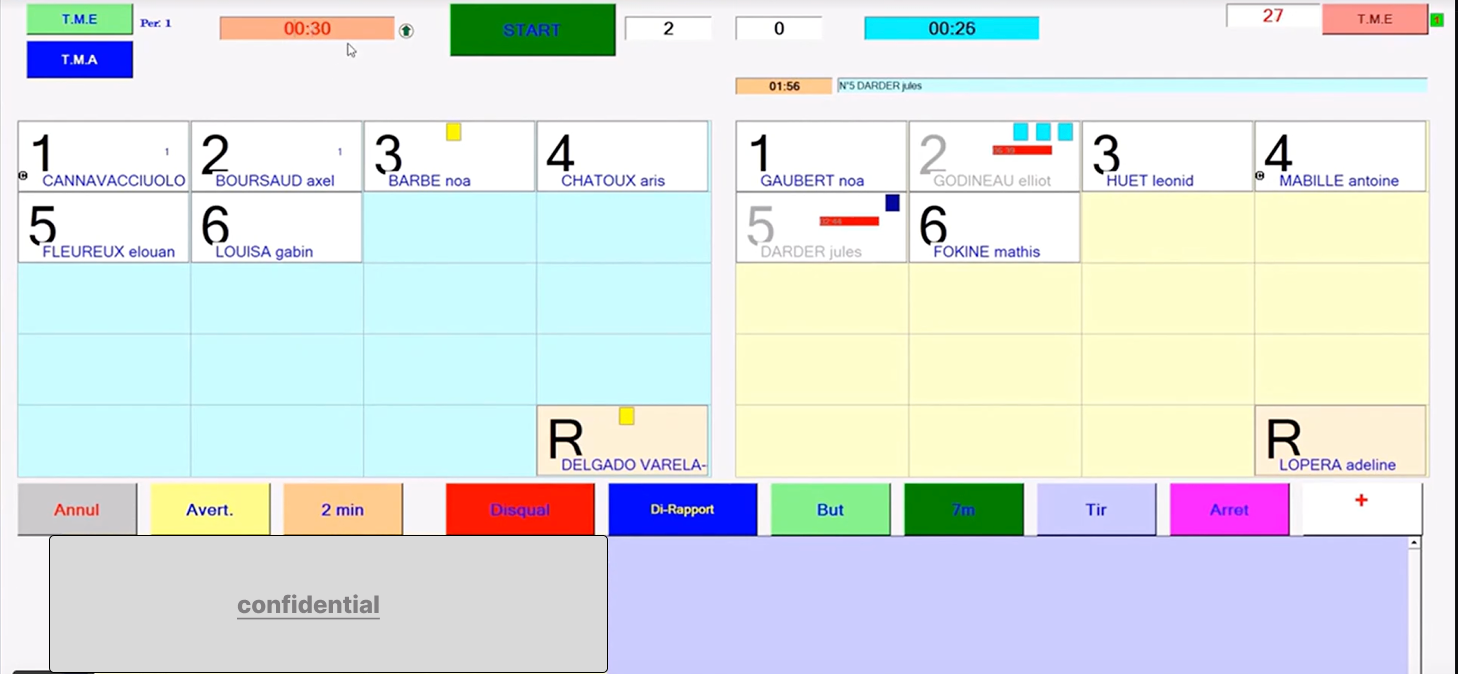
\includegraphics[width=12cm]{./images/legacy-system.png}
\caption{FDME Legacy App}
\end{figure}

\subsection{Technical Limitations and Performance Issues}

By 2025, the legacy FDME's technical limitations had become critical bottlenecks:
Platform Compatibility: The system required specific Windows versions and browser configurations that were increasingly difficult to maintain across the federation's diverse hardware ecosystem. Clubs struggled with compatibility issues on older machines, while newer devices often lacked necessary legacy components.

\textbf{Connectivity Resilience}: The original architecture assumed reliable internet connectivity, which was rarely available in sports venues. When connections failed, data could be lost or corrupted, requiring manual intervention and creating significant administrative overhead.

\textbf{User Interface Limitations}: The interface was designed for desktop use with mouse and keyboard input, making it difficult to use on tablets or touch devices that had become standard in many venues. Small buttons, complex navigation paths, and poor mobile responsiveness frustrated users and slowed match operations.

\textbf{Data Integrity Risks}: Limited validation rules and offline synchronization issues occasionally resulted in data inconsistencies, duplicate entries, or missing information that required manual correction by federation staff.

\textbf{Performance Degradation}: As match data volumes grew and user concurrency increased during peak weekend periods, the system experienced frequent slowdowns, timeouts, and crashes that disrupted live match operations.

\subsection{Real-World Operational Impact}

These technical limitations translated into tangible operational challenges that affected all stakeholders:

\textbf{Match Day Disruptions}: System failures during live matches created tense situations where referees couldn't record events, coaches couldn't verify player eligibility, and match results were delayed or lost entirely. In professional matches with television coverage, these delays could disrupt broadcast schedules and create contractual complications.

\textbf{Administrative Overhead}: Federation staff spent significant time manually resolving data inconsistencies, investigating missing match reports, and providing technical support to frustrated users. This reactive workload prevented investment in proactive improvements and strategic initiatives.

\textbf{User Frustration and Resistance}: Volunteers and officials increasingly expressed reluctance to use the system, with some reverting to paper-based processes that created additional manual data entry work for federation staff. This resistance threatened the federation's digital transformation goals and data quality objectives.

\textbf{Competitive Disadvantage}: While other national federations modernized their digital infrastructure, the federation's aging systems limited their ability to provide real-time statistics, enhanced broadcasting capabilities, and modern fan engagement features that had become standard in professional sports.


\subsection{Security and Compliance Concerns}

The legacy system's security architecture was designed for a different threat landscape and no longer met modern cybersecurity standards:

\textbf{Authentication Weaknesses}: Simple username/password authentication without multi-factor options created vulnerabilities, especially when credentials were shared among volunteers or stored insecurely.

\textbf{Audit Trail Limitations}: Insufficient logging and audit capabilities made it difficult to investigate data discrepancies, verify match results, or demonstrate compliance with regulatory requirements.



\section{Conclusion}

This chapter has established the comprehensive foundation necessary for understanding both the organizational excellence at Theodo Morocco and the complex challenges that necessitated the FDME modernization project. The intersection of Theodo's core values—rigor, pragmatism, eagerness to progress, and team spirit—with the federation's urgent need for digital transformation created an ideal environment for applying cutting-edge software engineering practices to challenges of national significance.
Theodo's evolution from Nimbleways into a key delivery hub within the international Theodo Group demonstrates the company's commitment to technical excellence and collaborative innovation. The comprehensive hiring process, from technical assessments through cultural alignment evaluation, and the structured onboarding experience reflect the organization's dedication to fostering professional growth while maintaining the highest standards of software delivery. These processes directly influenced how the FDME project was approached, ensuring that every team member was equipped with both the technical capabilities and collaborative mindset necessary for success.

The analysis of the National Sports Federation's operational scale—managing over 500,000 licensed members across 2,300 clubs and orchestrating more than 70,000 matches annually—reveals the critical importance of reliable digital infrastructure in modern sports administration. The federation's hierarchical structure, from elite professional leagues to grassroots youth development, creates complex reporting requirements that demand flexible, extensible technological solutions capable of adapting to diverse sporting contexts while maintaining data consistency and regulatory compliance.

The comprehensive examination of the legacy FDME system's limitations provides clear justification for the modernization initiative. From platform compatibility issues and connectivity resilience problems to user interface constraints and security vulnerabilities, the technical debt accumulated over fifteen years had created tangible operational challenges affecting every stakeholder in the handball ecosystem. The documented impact—including match day disruptions, administrative overhead, user frustration, and competitive disadvantage—demonstrates how technical limitations can directly undermine organizational effectiveness and user satisfaction.

Most importantly, this chapter establishes how Theodo's methodical approach to software delivery perfectly aligned with the federation's need for reliable, user-centered solutions. The company's emphasis on stakeholder collaboration, iterative development, and quality assurance provided the ideal framework for tackling the complex requirements of modernizing mission-critical systems while maintaining operational continuity. This foundation sets the stage for the detailed methodology, technical implementation, and successful outcomes that follow in subsequent chapters.

\newpage
